% Options for packages loaded elsewhere
% Options for packages loaded elsewhere
\PassOptionsToPackage{unicode}{hyperref}
\PassOptionsToPackage{hyphens}{url}
\PassOptionsToPackage{dvipsnames,svgnames,x11names}{xcolor}
%
\documentclass[
  letterpaper,
  DIV=11,
  numbers=noendperiod]{scrreprt}
\usepackage{xcolor}
\usepackage{amsmath,amssymb}
\setcounter{secnumdepth}{5}
\usepackage{iftex}
\ifPDFTeX
  \usepackage[T1]{fontenc}
  \usepackage[utf8]{inputenc}
  \usepackage{textcomp} % provide euro and other symbols
\else % if luatex or xetex
  \usepackage{unicode-math} % this also loads fontspec
  \defaultfontfeatures{Scale=MatchLowercase}
  \defaultfontfeatures[\rmfamily]{Ligatures=TeX,Scale=1}
\fi
\usepackage{lmodern}
\ifPDFTeX\else
  % xetex/luatex font selection
\fi
% Use upquote if available, for straight quotes in verbatim environments
\IfFileExists{upquote.sty}{\usepackage{upquote}}{}
\IfFileExists{microtype.sty}{% use microtype if available
  \usepackage[]{microtype}
  \UseMicrotypeSet[protrusion]{basicmath} % disable protrusion for tt fonts
}{}
\makeatletter
\@ifundefined{KOMAClassName}{% if non-KOMA class
  \IfFileExists{parskip.sty}{%
    \usepackage{parskip}
  }{% else
    \setlength{\parindent}{0pt}
    \setlength{\parskip}{6pt plus 2pt minus 1pt}}
}{% if KOMA class
  \KOMAoptions{parskip=half}}
\makeatother
% Make \paragraph and \subparagraph free-standing
\makeatletter
\ifx\paragraph\undefined\else
  \let\oldparagraph\paragraph
  \renewcommand{\paragraph}{
    \@ifstar
      \xxxParagraphStar
      \xxxParagraphNoStar
  }
  \newcommand{\xxxParagraphStar}[1]{\oldparagraph*{#1}\mbox{}}
  \newcommand{\xxxParagraphNoStar}[1]{\oldparagraph{#1}\mbox{}}
\fi
\ifx\subparagraph\undefined\else
  \let\oldsubparagraph\subparagraph
  \renewcommand{\subparagraph}{
    \@ifstar
      \xxxSubParagraphStar
      \xxxSubParagraphNoStar
  }
  \newcommand{\xxxSubParagraphStar}[1]{\oldsubparagraph*{#1}\mbox{}}
  \newcommand{\xxxSubParagraphNoStar}[1]{\oldsubparagraph{#1}\mbox{}}
\fi
\makeatother

\usepackage{color}
\usepackage{fancyvrb}
\newcommand{\VerbBar}{|}
\newcommand{\VERB}{\Verb[commandchars=\\\{\}]}
\DefineVerbatimEnvironment{Highlighting}{Verbatim}{commandchars=\\\{\}}
% Add ',fontsize=\small' for more characters per line
\usepackage{framed}
\definecolor{shadecolor}{RGB}{241,243,245}
\newenvironment{Shaded}{\begin{snugshade}}{\end{snugshade}}
\newcommand{\AlertTok}[1]{\textcolor[rgb]{0.68,0.00,0.00}{#1}}
\newcommand{\AnnotationTok}[1]{\textcolor[rgb]{0.37,0.37,0.37}{#1}}
\newcommand{\AttributeTok}[1]{\textcolor[rgb]{0.40,0.45,0.13}{#1}}
\newcommand{\BaseNTok}[1]{\textcolor[rgb]{0.68,0.00,0.00}{#1}}
\newcommand{\BuiltInTok}[1]{\textcolor[rgb]{0.00,0.23,0.31}{#1}}
\newcommand{\CharTok}[1]{\textcolor[rgb]{0.13,0.47,0.30}{#1}}
\newcommand{\CommentTok}[1]{\textcolor[rgb]{0.37,0.37,0.37}{#1}}
\newcommand{\CommentVarTok}[1]{\textcolor[rgb]{0.37,0.37,0.37}{\textit{#1}}}
\newcommand{\ConstantTok}[1]{\textcolor[rgb]{0.56,0.35,0.01}{#1}}
\newcommand{\ControlFlowTok}[1]{\textcolor[rgb]{0.00,0.23,0.31}{\textbf{#1}}}
\newcommand{\DataTypeTok}[1]{\textcolor[rgb]{0.68,0.00,0.00}{#1}}
\newcommand{\DecValTok}[1]{\textcolor[rgb]{0.68,0.00,0.00}{#1}}
\newcommand{\DocumentationTok}[1]{\textcolor[rgb]{0.37,0.37,0.37}{\textit{#1}}}
\newcommand{\ErrorTok}[1]{\textcolor[rgb]{0.68,0.00,0.00}{#1}}
\newcommand{\ExtensionTok}[1]{\textcolor[rgb]{0.00,0.23,0.31}{#1}}
\newcommand{\FloatTok}[1]{\textcolor[rgb]{0.68,0.00,0.00}{#1}}
\newcommand{\FunctionTok}[1]{\textcolor[rgb]{0.28,0.35,0.67}{#1}}
\newcommand{\ImportTok}[1]{\textcolor[rgb]{0.00,0.46,0.62}{#1}}
\newcommand{\InformationTok}[1]{\textcolor[rgb]{0.37,0.37,0.37}{#1}}
\newcommand{\KeywordTok}[1]{\textcolor[rgb]{0.00,0.23,0.31}{\textbf{#1}}}
\newcommand{\NormalTok}[1]{\textcolor[rgb]{0.00,0.23,0.31}{#1}}
\newcommand{\OperatorTok}[1]{\textcolor[rgb]{0.37,0.37,0.37}{#1}}
\newcommand{\OtherTok}[1]{\textcolor[rgb]{0.00,0.23,0.31}{#1}}
\newcommand{\PreprocessorTok}[1]{\textcolor[rgb]{0.68,0.00,0.00}{#1}}
\newcommand{\RegionMarkerTok}[1]{\textcolor[rgb]{0.00,0.23,0.31}{#1}}
\newcommand{\SpecialCharTok}[1]{\textcolor[rgb]{0.37,0.37,0.37}{#1}}
\newcommand{\SpecialStringTok}[1]{\textcolor[rgb]{0.13,0.47,0.30}{#1}}
\newcommand{\StringTok}[1]{\textcolor[rgb]{0.13,0.47,0.30}{#1}}
\newcommand{\VariableTok}[1]{\textcolor[rgb]{0.07,0.07,0.07}{#1}}
\newcommand{\VerbatimStringTok}[1]{\textcolor[rgb]{0.13,0.47,0.30}{#1}}
\newcommand{\WarningTok}[1]{\textcolor[rgb]{0.37,0.37,0.37}{\textit{#1}}}

\usepackage{longtable,booktabs,array}
\newcounter{none} % for unnumbered tables
\usepackage{calc} % for calculating minipage widths
% Correct order of tables after \paragraph or \subparagraph
\usepackage{etoolbox}
\makeatletter
\patchcmd\longtable{\par}{\if@noskipsec\mbox{}\fi\par}{}{}
\makeatother
% Allow footnotes in longtable head/foot
\IfFileExists{footnotehyper.sty}{\usepackage{footnotehyper}}{\usepackage{footnote}}
\makesavenoteenv{longtable}
\usepackage{graphicx}
\makeatletter
\newsavebox\pandoc@box
\newcommand*\pandocbounded[1]{% scales image to fit in text height/width
  \sbox\pandoc@box{#1}%
  \Gscale@div\@tempa{\textheight}{\dimexpr\ht\pandoc@box+\dp\pandoc@box\relax}%
  \Gscale@div\@tempb{\linewidth}{\wd\pandoc@box}%
  \ifdim\@tempb\p@<\@tempa\p@\let\@tempa\@tempb\fi% select the smaller of both
  \ifdim\@tempa\p@<\p@\scalebox{\@tempa}{\usebox\pandoc@box}%
  \else\usebox{\pandoc@box}%
  \fi%
}
% Set default figure placement to htbp
\def\fps@figure{htbp}
\makeatother





\setlength{\emergencystretch}{3em} % prevent overfull lines

\providecommand{\tightlist}{%
  \setlength{\itemsep}{0pt}\setlength{\parskip}{0pt}}



 


\KOMAoption{captions}{tableheading}
\makeatletter
\@ifpackageloaded{tcolorbox}{}{\usepackage[skins,breakable]{tcolorbox}}
\@ifpackageloaded{fontawesome5}{}{\usepackage{fontawesome5}}
\definecolor{quarto-callout-color}{HTML}{909090}
\definecolor{quarto-callout-note-color}{HTML}{0758E5}
\definecolor{quarto-callout-important-color}{HTML}{CC1914}
\definecolor{quarto-callout-warning-color}{HTML}{EB9113}
\definecolor{quarto-callout-tip-color}{HTML}{00A047}
\definecolor{quarto-callout-caution-color}{HTML}{FC5300}
\definecolor{quarto-callout-color-frame}{HTML}{acacac}
\definecolor{quarto-callout-note-color-frame}{HTML}{4582ec}
\definecolor{quarto-callout-important-color-frame}{HTML}{d9534f}
\definecolor{quarto-callout-warning-color-frame}{HTML}{f0ad4e}
\definecolor{quarto-callout-tip-color-frame}{HTML}{02b875}
\definecolor{quarto-callout-caution-color-frame}{HTML}{fd7e14}
\makeatother
\makeatletter
\@ifpackageloaded{bookmark}{}{\usepackage{bookmark}}
\makeatother
\makeatletter
\@ifpackageloaded{caption}{}{\usepackage{caption}}
\AtBeginDocument{%
\ifdefined\contentsname
  \renewcommand*\contentsname{Table of contents}
\else
  \newcommand\contentsname{Table of contents}
\fi
\ifdefined\listfigurename
  \renewcommand*\listfigurename{List of Figures}
\else
  \newcommand\listfigurename{List of Figures}
\fi
\ifdefined\listtablename
  \renewcommand*\listtablename{List of Tables}
\else
  \newcommand\listtablename{List of Tables}
\fi
\ifdefined\figurename
  \renewcommand*\figurename{Figure}
\else
  \newcommand\figurename{Figure}
\fi
\ifdefined\tablename
  \renewcommand*\tablename{Table}
\else
  \newcommand\tablename{Table}
\fi
}
\@ifpackageloaded{float}{}{\usepackage{float}}
\floatstyle{ruled}
\@ifundefined{c@chapter}{\newfloat{codelisting}{h}{lop}}{\newfloat{codelisting}{h}{lop}[chapter]}
\floatname{codelisting}{Listing}
\newcommand*\listoflistings{\listof{codelisting}{List of Listings}}
\makeatother
\makeatletter
\makeatother
\makeatletter
\@ifpackageloaded{caption}{}{\usepackage{caption}}
\@ifpackageloaded{subcaption}{}{\usepackage{subcaption}}
\makeatother
\usepackage{bookmark}
\IfFileExists{xurl.sty}{\usepackage{xurl}}{} % add URL line breaks if available
\urlstyle{same}
\hypersetup{
  pdftitle={HHS627 Textbook2},
  pdfauthor={Dr.~Andy Supple},
  colorlinks=true,
  linkcolor={blue},
  filecolor={Maroon},
  citecolor={Blue},
  urlcolor={Blue},
  pdfcreator={LaTeX via pandoc}}


\title{HHS627 Textbook2}
\author{Dr.~Andy Supple}
\date{2026-08-04}
\begin{document}
\maketitle

\renewcommand*\contentsname{Table of contents}
{
\setcounter{tocdepth}{2}
\tableofcontents
}

\bookmarksetup{startatroot}

\chapter*{Preface}\label{preface}
\addcontentsline{toc}{chapter}{Preface}

\markboth{Preface}{Preface}

This is a Quarto book.

To learn more about Quarto books visit
\url{https://quarto.org/docs/books}.

\begin{Shaded}
\begin{Highlighting}[]
\DecValTok{1} \SpecialCharTok{+} \DecValTok{1}
\end{Highlighting}
\end{Shaded}

\begin{verbatim}
[1] 2
\end{verbatim}

\bookmarksetup{startatroot}

\chapter{Chapter 1 HHS Statistical
Thinking}\label{chapter-1-hhs-statistical-thinking}

\bookmarksetup{startatroot}

\chapter{Statistical Thinking and Quantitative
Analysis}\label{statistical-thinking-and-quantitative-analysis}

\bookmarksetup{startatroot}

\chapter{Goals of Quantitative HHS
Research}\label{goals-of-quantitative-hhs-research}

Most quantitative HHS research seeks to:

\begin{itemize}
\tightlist
\item
  Describe populations and samples - descriptive purpose
\item
  Compare groups - understand differences, evaluate
  programs/interventions
\item
  Examine relationships among variables - how variables associate
\item
  Evaluate models with multiple predictors - what factors are most
  important in predicting outcomes
\end{itemize}

Researchers typically draw conclusions using statistical tests that
assess:

\begin{itemize}
\tightlist
\item
  Group differences
\item
  Correlations
\item
  Statistical significance
\end{itemize}

\bookmarksetup{startatroot}

\chapter{What Is Statistical
Significance?}\label{what-is-statistical-significance}

Statistical significance addresses a simple question:

\begin{quote}
Is the observed effect large enough that it is unlikely to be zero in
the population?
\end{quote}

Examples:

\begin{itemize}
\tightlist
\item
  Are males and females different in IQ?
\item
  Is father involvement related to girls' self-esteem?
\item
  Is the observed correlation different from zero? Is the difference so
  big, it is unlikely to be zero
\end{itemize}

\bookmarksetup{startatroot}

\chapter{Null Hypothesis Testing}\label{null-hypothesis-testing}

The null hypothesis states that no effect exists

Examples:

\begin{itemize}
\tightlist
\item
  No difference between groups
\item
  Correlation equals zero
\item
  Treatment effect equals zero
\end{itemize}

Statistical testing attempts to determine whether there is sufficient
evidence to reject the null hypothesis. So in your thesis/dissertation,
you are \emph{hoping} for \textbf{p} \textless.05 so you can ``reject
the null''

\bookmarksetup{startatroot}

\chapter{Type I Error}\label{type-i-error}

A Type I error occurs when:

\begin{itemize}
\tightlist
\item
  We reject the null hypothesis when null hypothesis is actually true
\end{itemize}

This is a false positive. We claim based on the data we collected from a
sample, that an effect exists

\begin{itemize}
\item
  High intensity interval training improves cardiovascular performance
  better than\ldots{}
\item
  Spanking/physical punishment is associated with increased aggressive
  behaviors in children\ldots{}
\item
  Smoking is related to stress\ldots{}
\item
  \textbf{\emph{But in the population those effects/differences don't
  exist/aren't true}}
\end{itemize}

The probability of committing a Type I error is determined by α (alpha),
typically:

\begin{itemize}
\tightlist
\item
  .05
\item
  .01
\item
  .001
\end{itemize}

\bookmarksetup{startatroot}

\chapter{Type II Error}\label{type-ii-error}

A Type II error occurs when:

\begin{itemize}
\tightlist
\item
  We fail to reject the null hypothesis when a real effect actually
  exists

  \begin{itemize}
  \tightlist
  \item
    Researcher concludes that UNCG women soccer players not more likely
    to experience ACL tears compared to male soccer players but in
    reality that is true in the population\ldots{}
  \item
    Children in classrooms with smaller teacher-to-student ratio do not
    have higher reading scores\ldots{}
  \item
    Frequency of smoking is not associated with lung cancer\ldots{}
  \end{itemize}
\end{itemize}

Common causes include:

\begin{itemize}
\tightlist
\item
  Small sample sizes
\item
  \textbf{Low statistical power}
\end{itemize}

\begin{figure}[H]

{\centering \pandocbounded{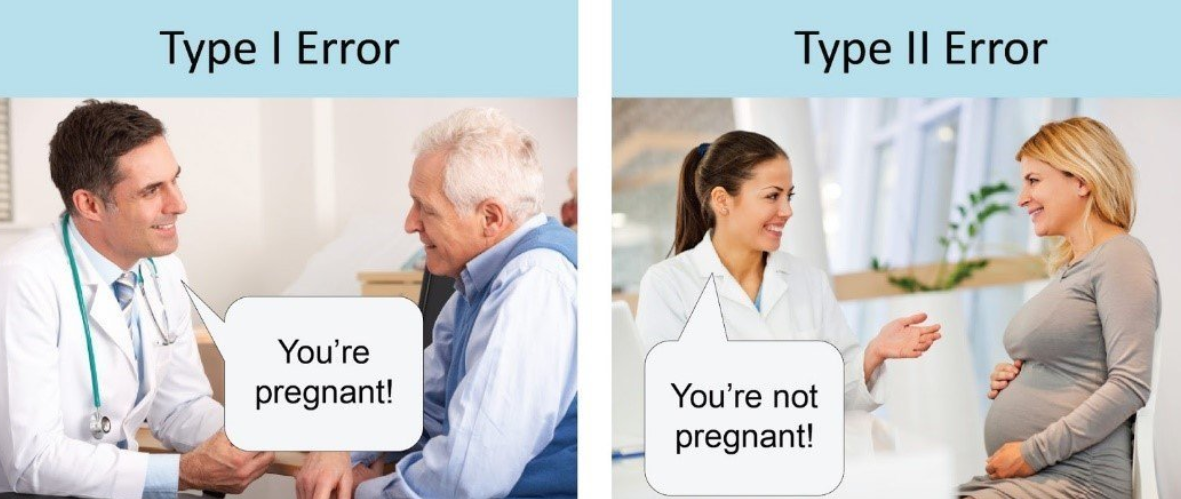
\includegraphics[keepaspectratio,alt={A Dr. Pointing to a man\textquotesingle s stomach and saying "you are pregnant" representing TYPE I error, a female Dr. pointing to an obviously pregnant woman\textquotesingle s belly and saying "you are not pregnant" to represent TYPE II error}]{images/Type Errors.png}}

}

\caption{Type I Type II Errors}

\end{figure}%

\bookmarksetup{startatroot}

\chapter{Problems with NHST}\label{problems-with-nhst}

Critics argue that:

\begin{itemize}
\tightlist
\item
  Virtually all null hypotheses are false and \textbf{illogical anyway}
\item
  p-values are often misinterpreted; not \textbf{95 chance the
  hypothesis is true}
\item
  Statistical significance says little about \emph{practical importance}
\item
  Lower p-values do not imply stronger effects
\end{itemize}

\begin{tcolorbox}[enhanced jigsaw, arc=.35mm, bottomrule=.15mm, bottomtitle=1mm, breakable, colback=white, colbacktitle=quarto-callout-note-color!10!white, colframe=quarto-callout-note-color-frame, coltitle=black, left=2mm, leftrule=.75mm, opacityback=0, opacitybacktitle=0.6, rightrule=.15mm, title=\textcolor{quarto-callout-note-color}{\faInfo}\hspace{0.5em}{Ban on p-values?}, titlerule=0mm, toprule=.15mm, toptitle=1mm]

\begin{itemize}
\tightlist
\item
  Statistical associations offer \textbf{severe critiques}
\item
  Some journals attempted to ban p-values!
\item
  \href{https://www.amstat.org/asa/files/pdfs/P-ValueStatement.pdf}{ASA
  Statement on p-values}
\item
  \href{http://www.stat.yale.edu/~jtc5/238/readings/Psychology-journal-bans-P-values_Nature.pdf}{Psych
  journal bans p-values (Nature, optional reading)}
\end{itemize}

\end{tcolorbox}

Researchers increasingly advocate reporting:

\begin{itemize}
\tightlist
\item
  Effect sizes
\item
  Confidence intervals
\item
  Bayesian analyses - what is this?
\end{itemize}

\bookmarksetup{startatroot}

\chapter{Statistical versus Practical
Significance}\label{statistical-versus-practical-significance}

A statistically significant effect may be trivial in practice

Large samples can make tiny effects statistically significant

\begin{itemize}
\tightlist
\item
  Do I want to encourage schools to target suicide prevention to
  Southeast Asian students based on 8.5\% self-reported suicidal
  thoughts were 8.9\%?
\end{itemize}

Therefore researchers should report:

\begin{itemize}
\tightlist
\item
  Effect sizes
\item
  Confidence intervals
\item
  Practical implications
\end{itemize}

\bookmarksetup{startatroot}

\chapter{Quick Review of some other
terms/ideas/stats}\label{quick-review-of-some-other-termsideasstats}

\bookmarksetup{startatroot}

\chapter{Confidence Intervals}\label{confidence-intervals}

\section{Confidence Intervals}\label{confidence-intervals-1}

\begin{itemize}
\tightlist
\item
  Confidence intervals estimate a plausible range of values for a
  population parameter
\item
  A \textbf{parameter} is a population value; a \textbf{statistic} is
  what we calculate from a sample to estimate that parameter
\item
  Typically we estimate something like a regression coefficient and want
  to assess whether that coefficient differs from zero
\item
  If we put a confidence interval around that coefficient and the
  interval does \textbf{not} include zero, that indicates statistical
  significance (using a \emph{p} \textless{} .05 threshold)
\item
  If the interval \textbf{does} include zero, we cannot rule out that
  the true population value is zero --- not statistically significant
\end{itemize}

\begin{tcolorbox}[enhanced jigsaw, arc=.35mm, bottomrule=.15mm, bottomtitle=1mm, breakable, colback=white, colbacktitle=quarto-callout-tip-color!10!white, colframe=quarto-callout-tip-color-frame, coltitle=black, left=2mm, leftrule=.75mm, opacityback=0, opacitybacktitle=0.6, rightrule=.15mm, title=\textcolor{quarto-callout-tip-color}{\faLightbulb}\hspace{0.5em}{Rule of Thumb}, titlerule=0mm, toprule=.15mm, toptitle=1mm]

A 95\% confidence interval that excludes zero typically indicates
statistical significance at the \emph{p} \textless{} .05 level.

\end{tcolorbox}

\subsection{Visualizing Confidence
Intervals}\label{visualizing-confidence-intervals}

\begin{figure}[H]

{\centering \pandocbounded{
\includegraphics[keepaspectratio]{Chapter-1-HHS-Statistical-Thinking_files/figure-pdf/unnamed-chunk-1-1.pdf}}

}

\caption{Example confidence intervals: one significant (excludes zero),
one not significant (includes zero)}

\end{figure}%

\bookmarksetup{startatroot}

\chapter{Standardized (Z) Scores}\label{standardized-z-scores}

Z scores place observations on a common scale

Formula:

\[z=\frac{X-\bar X}{SD}\]

Interpretation:

\begin{itemize}
\tightlist
\item
  Positive z = above the mean
\item
  Negative z = below the mean
\end{itemize}

Example:

A score of 78 may be above average in one class but below average in
another

Z scores place both scores in context

\bookmarksetup{startatroot}

\chapter{Part II: Choosing an
Analysis}\label{part-ii-choosing-an-analysis}

Questions to consider:

\begin{enumerate}
\def\labelenumi{\arabic{enumi}.}
\tightlist
\item
  What is the research question?
\item
  What is the hypothesis?
\item
  What is the research design?
\item
  How many variables are involved?
\item
  What levels of measurement are present?
\end{enumerate}

\section{What is the Research Question and
Hypotheses}\label{what-is-the-research-question-and-hypotheses}

The Research Question and Hypotheses make a statement about how we see
some human phenomenon.

\begin{itemize}
\item
  RQ: Are there gender differences in suicidal thoughts?

  \begin{itemize}
  \tightlist
  \item
    HYP: Girls are more likely than boys to have suicidal thoughts
  \end{itemize}
\end{itemize}

This hypothesis also implies a research design as this would be a
comparative study with no random assignments

\section{What is the Research
Design?}\label{what-is-the-research-design}

Is my study an experiment? A quasi-experiment? Comparing groups?

\begin{itemize}
\tightlist
\item
  Those types of research designs tend to imply that there is a factor
  or categorical Independent Variable (IV) across which I expect to find
  a difference across groups of people
\end{itemize}

Am I considering associational or correlational relationships? Am I
expecting that participants who score higher on one variable also tend
to score higher on a second variable?

\begin{itemize}
\tightlist
\item
  Are college students who report higher experiences with discrimination
  from peers more likely to report feelings of anxiety?
\end{itemize}

This would imply an associational design with no factor/categorical
variables, attribute variables (something participants ``bring'' with
them into the study, unlike an ``active'' IV)

\section{How many variables are
involved?}\label{how-many-variables-are-involved}

\bookmarksetup{startatroot}

\chapter{Group Comparison Tests}\label{group-comparison-tests}

Any group comparison test typically follows an hypothesis that proposes
that one group of people (that we might think of as a sub population of
people - or units, whatever we are studying) scores higher on some
outcome compared to another group of people.

Sometimes the groups under consideration can really be from one
population, but some experimental manipulation is imposed on one group
and that same manipulation is withheld from the other group.

The \textbf{classic experimental design} with \emph{random assignment}
would create differences among theoretically equivalence groups and has
strong \emph{internal validity} because any differences in groups later
on (after some intervention or manipulation)

\begin{itemize}
\tightlist
\item
  That is a group comparison!
\end{itemize}

Are college students who visit their respective Student Recreation
Centers more connected to their campus?

\begin{itemize}
\item
  If we could assess some scores with an average score on ``campus
  connection''
\item
  Then we would be interested to see if those scores were different, and
  if so, by a big enough amount to claim those differences as
  meaningfully important
\item
  We use the term \emph{statistically significant\ldots{}}
\end{itemize}

\textbf{Independent Samples t Test}

\begin{itemize}
\tightlist
\item
  Used to compare means (so continuous variables) across two groups
\end{itemize}

Examples:

\begin{itemize}
\tightlist
\item
  Men versus women: Do women report greater parental anxiety than men?
\item
  Treatment versus control: Do participants in a smoking cessation
  program\ldots{}
\end{itemize}

\textbf{ANOVA}

-Used to compare means across three or more groups

\textbf{ANCOVA}

-ANOVA including covariates, or control variables

\textbf{MANOVA}

Multiple dependent variables

\bookmarksetup{startatroot}

\chapter{Tests of Association}\label{tests-of-association}

\textbf{Pearson Correlation}

Used with two continuous variables

Examples:

\begin{itemize}
\tightlist
\item
  Age and self-esteem
\item
  Education and income
\end{itemize}

Other Correlations

\begin{itemize}
\tightlist
\item
  Kendall's Tau
\item
  Polychoric
\item
  Polyserial
\item
  Point-biserial
\item
  Phi
\end{itemize}

\bookmarksetup{startatroot}

\chapter{Multiple Regression}\label{multiple-regression}

Multiple regression predicts one outcome from multiple predictors

General model:

\[Y = a + b_1X_1 + b_2X_2 + e\]

Researchers use regression to:

\begin{itemize}
\tightlist
\item
  Explain phenomena
\item
  Control for confounding variables
\item
  Estimate unique effects of predictors
\end{itemize}

\bookmarksetup{startatroot}

\chapter{Logistic Regression}\label{logistic-regression}

Used when the outcome variable is dichotomous

Examples:

\begin{itemize}
\tightlist
\item
  Pregnant/not pregnant
\item
  Used drugs/did not use drugs
\item
  Died/survived
\end{itemize}

Results typically include:

\begin{itemize}
\tightlist
\item
  Regression coefficients
\item
  Odds ratios
\end{itemize}

\bookmarksetup{startatroot}

\chapter{Correlation versus
Regression}\label{correlation-versus-regression}

Correlation addresses association

Regression allows:

\begin{itemize}
\tightlist
\item
  Multiple predictors
\item
  Statistical control
\item
  Prediction
\end{itemize}

Example:

Divorce may predict adolescent depression, but that relation may weaken
after controlling for inter-parental conflict

\bookmarksetup{startatroot}

\chapter{Statistical Power and Effect
Size}\label{statistical-power-and-effect-size}

Power analysis helps determine sample size requirements

General rule:

\begin{itemize}
\tightlist
\item
  Large effects require smaller samples
\item
  Small effects require larger samples
\end{itemize}

Power analysis is especially important in grant writing

\bookmarksetup{startatroot}

\chapter{Quick Note}\label{quick-note}

There really is not a difference between ANOVAs and Regressions!

-There were historical reasons why ANOVA came to be associated with
experimental and agricultural research -Researchers used to think that
if one was doing experiments, they should do an ANOVA -If they were
doing observational/correlational research, should use regressions -I
was taught that in grad school at first, then in class taught that these
were all the \textbf{general linear model}

\bookmarksetup{startatroot}

\chapter{The General Linear Model}\label{the-general-linear-model}

This applies to any analysis that has a continuous (interval or ratio)
or ``quantitative'' outcome

-T-tests and ANOVAs are just a ``special'' case - that is, they are
regressions with a categorical predictor or IV or X - if you run a
t-test comparing self-esteem across boys/girls and then run a regression
where you regress self-esteem on gender (dummy coded) you will get the
same result! - Note I worked on a multisite project where the
statistician at the other institution was running ``ANCOVAs'' to
evaluate the intervention effect -That made sense because he was
considering how 6-month post-test anxiety (for example) differed by
group (experimental vs control), controlling for baseline scores -I did
the same exact analysis but called it a multiple regression, I regressed
6 month anxiety on an effects coded binary X or IV variable and
controlled for baseline anxiety -We would come to the same conclusion in
this case\ldots{}

The point of all of this is to say\ldots{}

\begin{itemize}
\tightlist
\item
  ANOVA
\end{itemize}




\end{document}
